\documentclass{standalone}

\usepackage[OT1]{fontenc}
\renewcommand*\familydefault{\sfdefault}
\usepackage{helvet,sfmath}
\usepackage{siunitx}

\usepackage{tikz}
\usetikzlibrary{arrows,calc,patterns}
% \usetikzlibrary{intersections, calc, arrows.meta}
\usepackage{tikz,tkz-euclide}
\begin{document}

    \centering
    \tikzset{every picture/.style={line width=0.75pt}} %set default line width to 0.75pt        

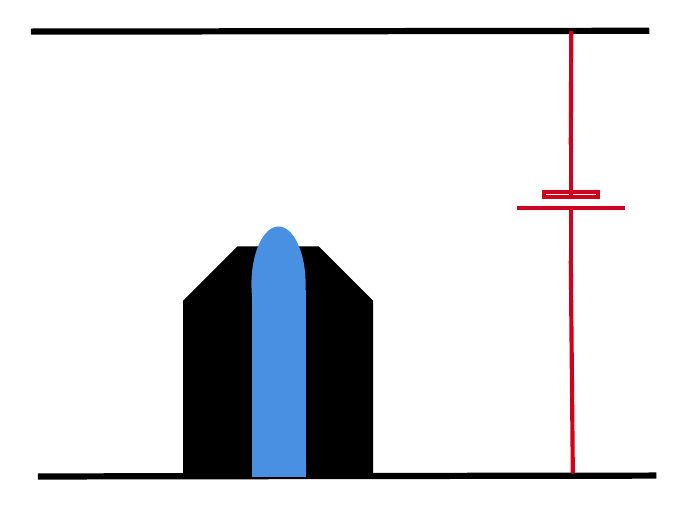
\begin{tikzpicture}[x=0.75pt,y=0.75pt,yscale=-1,xscale=1]
%uncomment if require: \path (0,300); %set diagram left start at 0, and has height of 300

%Straight Lines [id:da9645128262017965] 
\draw [line width=2.25]    (174.44,233) -- (472.41,232.59) ;
%Snip Same Side Corner Rect [id:dp90093720621791] 
\draw  [fill={rgb, 255:red, 0; green, 0; blue, 0 }  ,fill opacity=1 ] (244.62,148.49) -- (270.63,122.47) -- (309.66,122.47) -- (335.68,148.49) -- (335.68,232.16) -- (335.68,232.16) -- (244.62,232.16) -- (244.62,232.16) -- cycle ;
%Shape: Rectangle [id:dp1868800164119795] 
\draw  [draw opacity=0][fill={rgb, 255:red, 74; green, 144; blue, 226 }  ,fill opacity=1 ] (277.41,143.28) -- (303.41,143.28) -- (303.41,233.28) -- (277.41,233.28) -- cycle ;
%Straight Lines [id:da09766177709908785] 
\draw [color={rgb, 255:red, 208; green, 2; blue, 27 }  ,draw opacity=1 ][fill={rgb, 255:red, 208; green, 2; blue, 27 }  ,fill opacity=1 ][line width=1.5]    (431.17,128.98) -- (432.15,231.58) ;
%Shape: Battery [id:dp03651270276576213] 
\draw  [color={rgb, 255:red, 208; green, 2; blue, 27 }  ,draw opacity=1 ][line width=1.5]  (431.17,73.02) -- (431.17,98.21) (457.19,103.8) -- (405.15,103.8) (431.17,103.8) -- (431.17,128.98) (444.18,95.97) -- (444.18,98.21) -- (418.16,98.21) -- (418.16,95.97) -- (444.18,95.97) -- cycle ;
%Straight Lines [id:da8963203540020234] 
\draw [line width=2.25]    (171,18.68) -- (468.97,18.28) ;
%Shape: Chord [id:dp306499765403625] 
\draw  [draw opacity=0][fill={rgb, 255:red, 74; green, 144; blue, 226 }  ,fill opacity=1 ] (277.48,145.01) .. controls (277.36,143.49) and (277.3,141.92) .. (277.3,140.33) .. controls (277.3,125) and (283.14,112.57) .. (290.35,112.57) .. controls (297.56,112.57) and (303.41,125) .. (303.41,140.33) .. controls (303.41,141.92) and (303.34,143.49) .. (303.22,145.01) -- cycle ;
%Straight Lines [id:da9311566255922183] 
\draw [color={rgb, 255:red, 208; green, 2; blue, 27 }  ,draw opacity=1 ][fill={rgb, 255:red, 208; green, 2; blue, 27 }  ,fill opacity=1 ][line width=1.5]    (431.41,18.28) -- (431.17,73.02) ;
\end{tikzpicture}



\end{document}
